\chapter{Extended figure gallery}

This appendix collects the remaining result figures referenced by the
findings but not embedded in the main text, with interpretive captions.
Together with the in-text figures they constitute the complete graphic
record of the investigation.

\section{Kernel-band era and the full ladder}

\begin{figure}[H]\centering
  
\includegraphics[width=0.92\linewidth]{fl_figs/fig2_slope_deficit.png}
  \caption{Slope and deficit along the 1000-cell R4 DD ladder. These are
    the quantities later revised by the \strict{} recheck: the
    high-$\tau$ deficit rise is predominantly operator bias.}
\end{figure}

\begin{figure}[H]\centering
  
\includegraphics[width=0.92\linewidth]{fl_figs/fig4_Prange.png}
  \caption{Price range along the R4 ladder: the equilibrium sharpens
    with $\tau$ --- qualitatively robust across operators even where the
    deficit numbers are not.}
\end{figure}

\begin{figure}[H]\centering
  
\includegraphics[width=0.92\linewidth]{fl_figs/fig6_contours.png}
  \caption{R4 equilibrium contours across the ladder: the early visual
    evidence of the kink structure that the spectral and cusp analyses
    later formalized.}
\end{figure}

\begin{figure}[H]\centering
  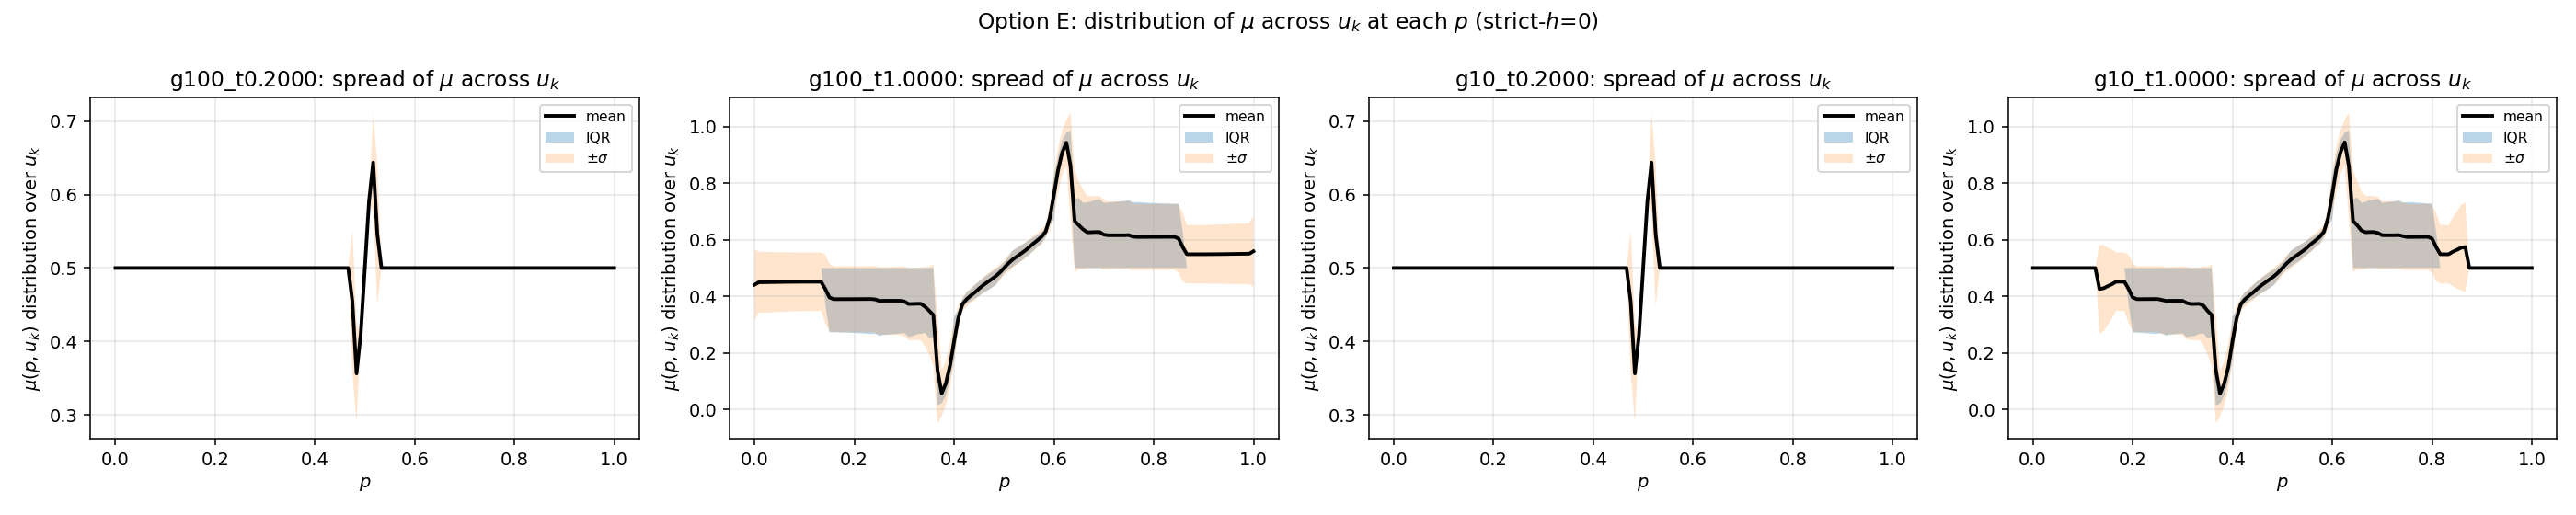
\includegraphics[width=0.85\linewidth]{alts_figs/fig4_distribution.png}
  \caption{Error distributions across the five lookup builders: Option
    B+ concentrates its mass two decades left of all kernel-band
    variants.}
\end{figure}

\begin{figure}[H]\centering
  
\includegraphics[width=0.92\linewidth]{optB_figs/fig2_sweep.png}
  \caption{Option B+ accuracy across $(\gamma, \tau)$: uniform in
    $\gamma$, mildly degrading at high $\tau$ as the cube CDF's tails
    thin.}
\end{figure}

\begin{figure}[H]\centering
  
\includegraphics[width=0.92\linewidth]{optB_figs/fig3_cross.png}
  \caption{Cross-sectional view: B+ tracks \strict{} to plotting
    accuracy at a representative cell.}
\end{figure}

\begin{figure}[H]\centering
  
\includegraphics[width=0.85\linewidth]{optD_figs/fig2_avg.png}
  \caption{Adaptive $p$-grid: average max-error by monitor function ---
    arclength wins consistently.}
\end{figure}

\section{Cusp geometry, continued}

\begin{figure}[H]\centering
  
\includegraphics[width=0.85\linewidth]{cusps_figs/fig1_grad_critical.png}
  \caption{Critical points on a second slice/regime, complementing the
    main-text figure: the critical manifold moves with $u_k$ ---
    the geometric root of Finding 13 (slice criticality, not 3D
    criticality, governs the lookup cusps).}
\end{figure}

\begin{figure}[H]\centering
  
\includegraphics[width=0.85\linewidth]{cusps_figs/fig1_mu_cusps.png}
  \caption{Lookup cusps for the slice of the previous figure.}
\end{figure}

\begin{figure}[H]\centering
  
\includegraphics[width=0.85\linewidth]{cusps_figs/fig4_regime.png}
  \caption{The smooth/cuspy regime boundary in $(\gamma, \tau)$:
    interior critical points (and hence lookup cusps) emerge with
    rising $\tau$; below the boundary global spectral methods would
    suffice.}
\end{figure}

\begin{figure}[H]\centering
  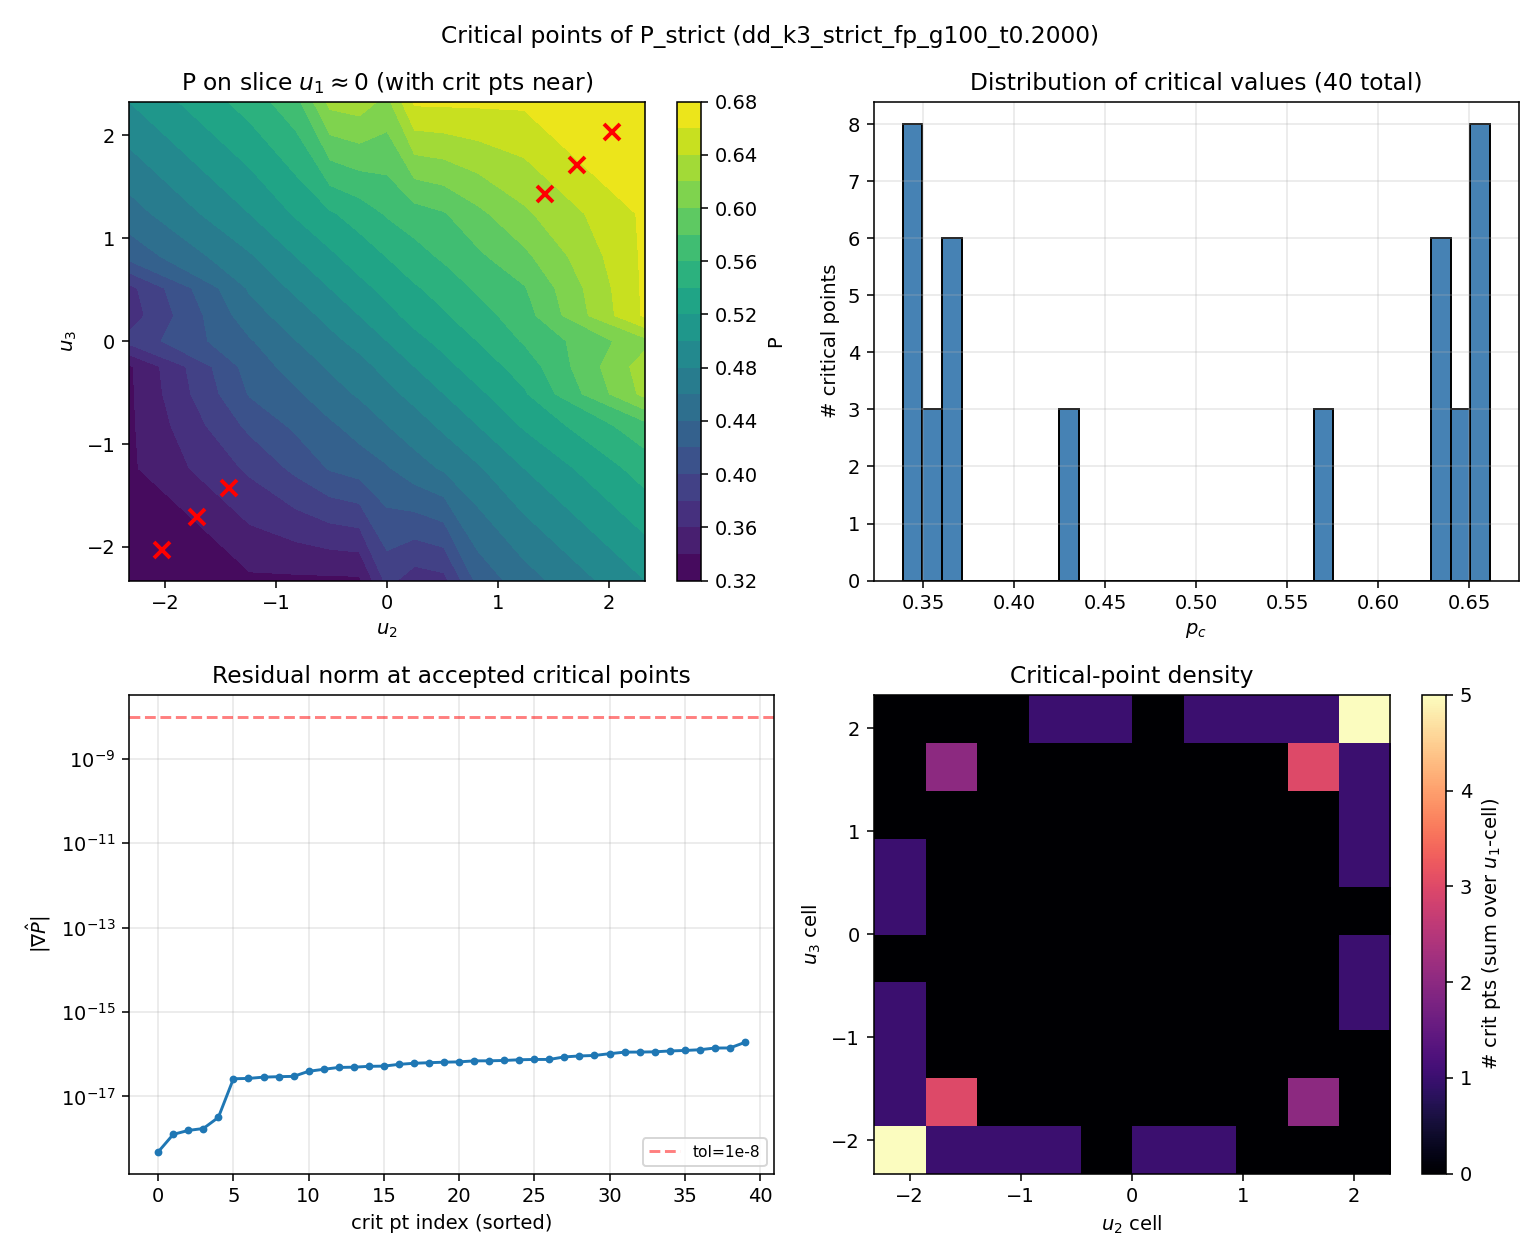
\includegraphics[width=0.8\linewidth]{critpts/dd_k3_strict_fp_g100_t0.2000.png}
  \caption{3D critical points at $(\gamma, \tau) = (100, 0.2)$: 40
    points, 16 unique critical values confined to $p \in [0.34, 0.66]$
    --- the narrower cusp band of the low-$\tau$ regime.}
\end{figure}

\begin{figure}[H]\centering
  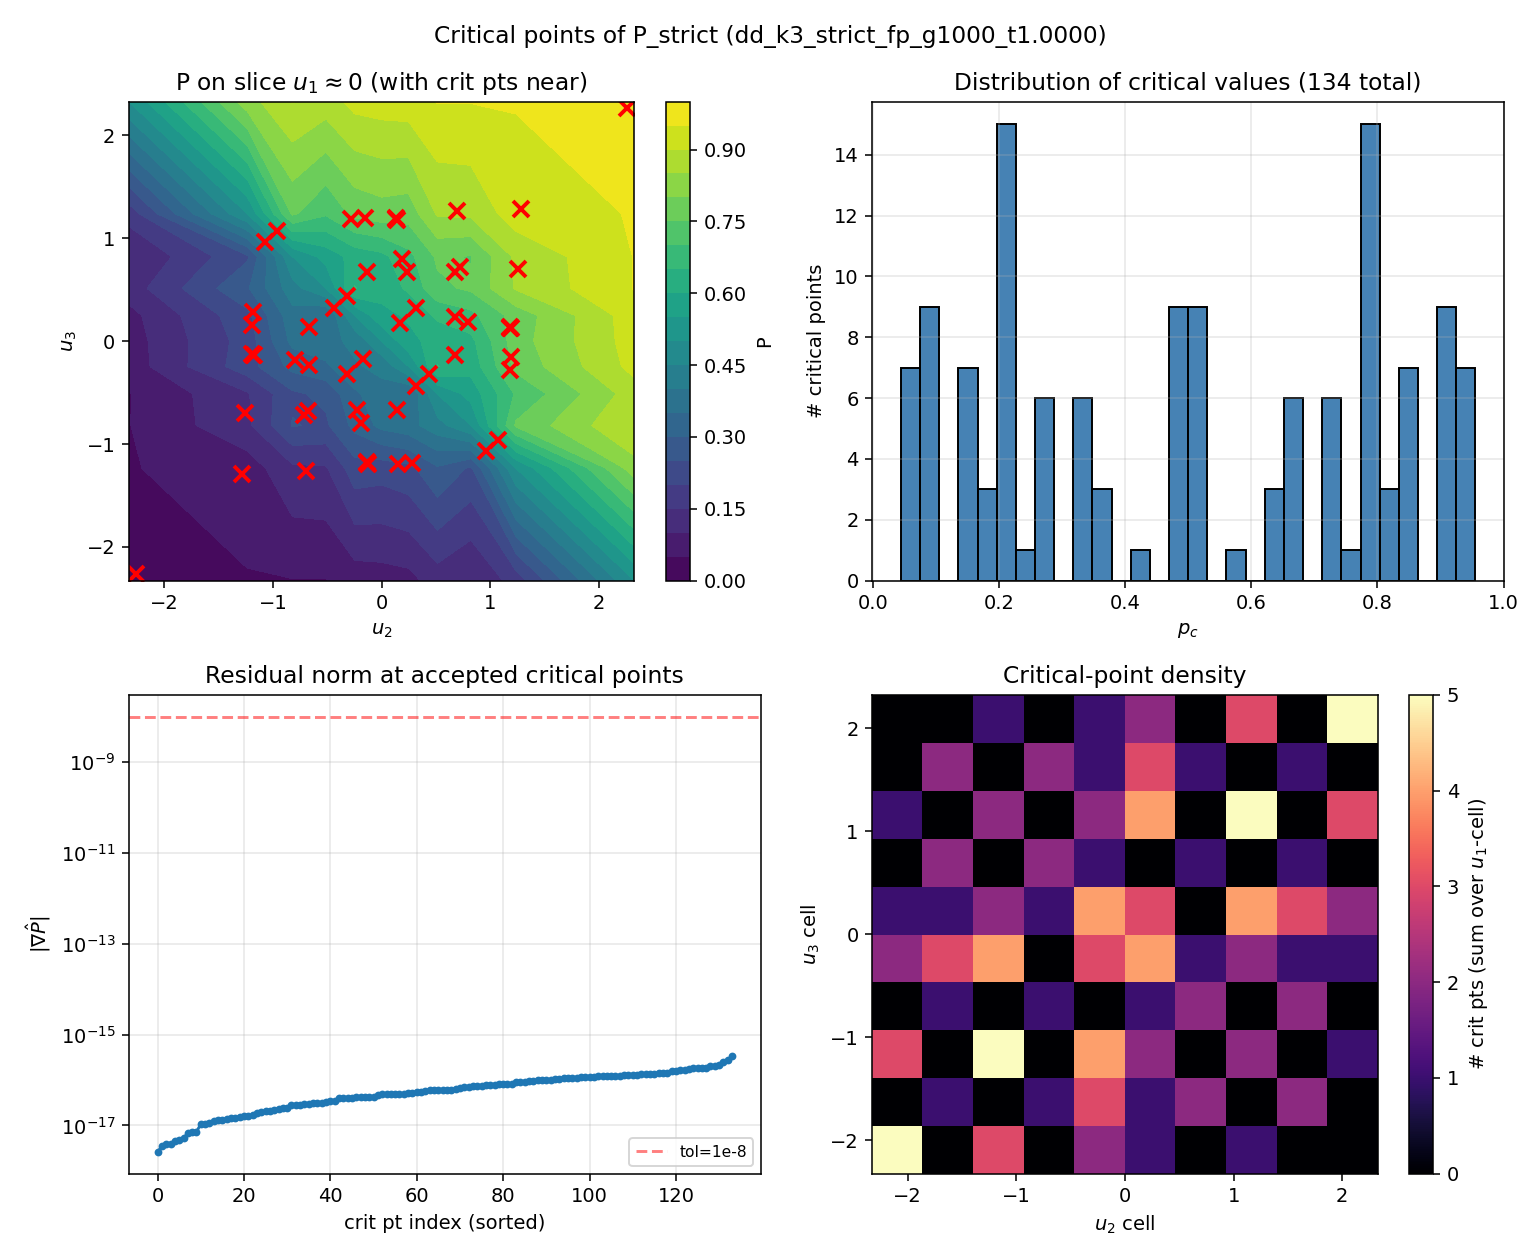
\includegraphics[width=0.8\linewidth]{critpts/dd_k3_strict_fp_g1000_t1.0000.png}
  \caption{3D critical points at $(\gamma, \tau) = (1000, 1)$: the
    high-$\gamma$, high-$\tau$ corner; 134 points spanning
    $p \in [0.05, 0.96]$.}
\end{figure}

\section{Structural ansatz, continued}

\begin{figure}[H]\centering
  
\includegraphics[width=0.9\linewidth]{mcv2_figs/fig3_Prange.png}
  \caption{Method C v2 ladder: price range vs $\tau$ under the additive
    ansatz --- smooth and monotone by construction.}
\end{figure}

\begin{figure}[H]\centering
  
\includegraphics[width=0.9\linewidth]{mcv2_figs/fig4_coefs.png}
  \caption{Evolution of the five ansatz coefficients along the
    $\tau$-ladder: smooth trajectories, suitable for warm-starting and
    for interpolating the ansatz across $\tau$.}
\end{figure}

\begin{figure}[H]\centering
  
\includegraphics[width=0.9\linewidth]{mcv2_figs/fig5_diag.png}
  \caption{Ansatz diagnostics along the ladder.}
\end{figure}

\begin{figure}[H]\centering
  
\includegraphics[width=0.9\linewidth]{mcv2t_figs/fig2_P_slices.png}
  \caption{Ansatz price slices at $\tau = 0.001$: visually
    indistinguishable from the analytic linear-Gaussian limit.}
\end{figure}

\begin{figure}[H]\centering
  
\includegraphics[width=0.85\linewidth]{mcv2g_figs/fig4_cross.png}
  \caption{Grid cross-sections: every $\gamma$ row shows the same
    $\tau$-transition --- the factorization
    $\|F\|(\gamma, \tau) \approx \|F\|(\tau)$ of the ansatz residual.}
\end{figure}

\begin{figure}[H]\centering
  
\includegraphics[width=0.9\linewidth]{mcv3_figs/fingerprint.png}
  \caption{The original v3 fingerprint (against the R4-era ansatz fit):
    diagonal and dissenter slices of the residual with candidate
    polynomial overlays --- the first evidence that no simple symmetric
    polynomial captures the non-additive structure.}
\end{figure}

\section{The pipeline iterations (v2--v4) and negative controls}

\begin{figure}[H]\centering
  
\includegraphics[width=0.9\linewidth]{v2_figs/g100_t1.0_deg6.png}
  \caption{Pipeline v2 at $(100, 1)$, degree 6: machine epsilon
    in-support, fallback plateau out-of-support (pre-tail-extrapolation
    stage).}
\end{figure}

\begin{figure}[H]\centering
  
\includegraphics[width=0.9\linewidth]{v3p_figs/g100_t1.0_deg6.png}
  \caption{Pipeline v3: Chebyshev tail extrapolation with Bayesian BCs
    --- boundary-correct but with degree-2 tail overshoot
    (non-monotone), motivating v4's PCHIP tails.}
\end{figure}

\begin{figure}[H]\centering
  
\includegraphics[width=0.9\linewidth]{v4_figs/g100_t1.0_deg6.png}
  \caption{Pipeline v4: shape-preserving tails. Monotone where the
    input is monotone --- which exposed that the raw input was not
    (the fallback artifact), leading to Finding 14.}
\end{figure}

\begin{figure}[H]\centering
  
\includegraphics[width=0.9\linewidth]{v5_figs/g1000_t1.0_deg6.png}
  \caption{Pipeline v5 at the $(1000, 1)$ corner: the full
    clean-detect-fit-extrapolate chain on the hardest reference cell.}
\end{figure}

\begin{figure}[H]\centering
  
\includegraphics[width=0.9\linewidth]{me_figs/g100_t1.0.png}
  \caption{Multi-element OptB+ (Finding 8): median pinned to zero at
    inserted knots, max unmoved --- the diagnosis that the max error
    lives in the tails, not at the bulk cusps.}
\end{figure}

\begin{figure}[H]\centering
  
\includegraphics[width=0.9\linewidth]{exact_figs/compare_g100_t1.0000.png}
  \caption{Exact cell-mass integration vs step summation (Finding 12)
    at $(100, 1)$: the in-support median halves; the tails do not
    improve.}
\end{figure}

\begin{figure}[H]\centering
  
\includegraphics[width=0.9\linewidth]{tail_figs/mu_curves_g100_t1.0.png}
  \caption{Tail-BC variants (Finding 11): baseline, BC-augmented,
    logit-space, and Beta-CDF lookups overlaid --- the three BC
    variants are indistinguishable from baseline in the bulk, and the
    bulk is where the max error lives.}
\end{figure}

\begin{figure}[H]\centering
  
\includegraphics[width=0.9\linewidth]{smooth_figs/stall_trace.png}
  \caption{The stall trace that opened Finding 9: damped Picard
    \emph{diverges from the saved ``fixed point''} at every damping
    tested --- proof that the saved \strict{} object was a best
    iterate.}
\end{figure}

\begin{figure}[H]\centering
  
\includegraphics[width=0.85\linewidth]{mono_figs/fig1_orig_vs_mono.png}
  \caption{Monotonicity projection experiment on the R4 fixed points:
    enforcing axis-monotonicity post hoc reshapes the surface
    materially --- corroborating that the R4 violations were not
    cosmetic.}
\end{figure}

\begin{figure}[H]\centering
  
\includegraphics[width=0.75\linewidth]{trf_figs/fig1_trf_conv.png}
  \caption{Trust-region convergence of the ansatz fit: quadratic basin
    behavior, hitting the ansatz expressiveness floor in tens of
    iterations --- solver speed was never the v2/v3 bottleneck.}
\end{figure}

\section{The log-odds configuration, continued}

\begin{figure}[H]\centering
  
\includegraphics[width=0.9\linewidth]{lo_figs/g100_t0.1000_G15.png}
  \caption{Log-odds configuration at $G = 15$: the weighted residual
    reaches $10^{-4}$ before the (frozen) $\Lpub$ refresh perturbs it
    --- the best surface obtained in the new coordinates at
    $\tau = 0.1$.}
\end{figure}

\begin{figure}[H]\centering
  
\includegraphics[width=0.9\linewidth]{lo_figs/g1_t0.1000_G11.png}
  \caption{$\gamma = 1$ in the log-odds configuration: the
    low-risk-aversion cell --- largest Jensen wedge, widest price
    range, and the noisiest convergence of the sweep, consistent with
    the $1/\gamma$ scaling of the curvature term.}
\end{figure}

\begin{figure}[H]\centering
  
\includegraphics[width=0.9\linewidth]{lo_figs/g1000_t0.1000_G11.png}
  \caption{$\gamma = 1000$: approaching the CARA limit --- tighter
    price function, cleaner convergence; the wedge shrinks as
    $1/\gamma$.}
\end{figure}
